\renewcommand\thesection{\Alph{section}}
\renewcommand\thesubsection{\thesection.\arabic{subsection}}
\setcounter{section}{5}
\section{Entrega final}

\setcounter{subsection}{1}
\subsection{Implementar el manejo de excepciones capturando errores potenciales específicos mediante Try-catch}

Se utiliza en reiteradas ocasiones la captura de excepciones que puedan surgir en el programa mediante los bloques try-catch que se detallan a continuación:

\begin{itemize}
    \item Excepciones de conexión con base de datos SQL (\textbf{SQLException})
    \begin{itemize}
        \item \mintinline{java}{public Map<String, Alumno> getAlumnos()}
        \item \mintinline{java}{public Map<String, Alumno> getAlumnos(int nivel)}
        \item \mintinline{java}{public Map<String, Alumno> getAlumnos(int nivel, char paralelo)}
        \item \mintinline{java}{public Alumno getAlumno(String rut)}
        \item \mintinline{java}{public RegistroAsistencia get(IDAsistencia id)}
        \item \mintinline{java}{public RegistroAsistencia getRegistroAsistencia(IDAsistencia id)}
        \item \mintinline{java}{public RegistroAsistencia getRegistroAsistencia(Date fecha)}
        \item \mintinline{java}{public RegistroAsistencia getRegistroAsistencia(String rutAlumno)}
        \item \mintinline{java}{public ResultSet getQuery(String sql)}
        \item \mintinline{java}{public ResultSet updateQuery(String sql)}
    \end{itemize}
\end{itemize}

Se utilizan los bloques try-catch ya que en cada uno de ellos existe la posibilidad de una excepcion con la conexión o las consultas a la base de datos generando un \textbf{SQLException} o un \textbf{SQLTimeoutException}, además los métodos getter utilizados dentro de estos métodos también podrían generar un \textbf{SQLException} o un \textbf{SQLFeatureNotSupportedException}.\\

En cuanto a los siguientes métodos, se utilizan bloques try-catch ya que al imprimir los distintos tipos de menú se pueden generar excepciones de tipo IOException en operaciones I/O fallidas o interrumpidas.

\begin{itemize}
    \item Excepciones de entrada/salida de datos por consola (\textbf{IOException})
    \begin{itemize}
        \item \mintinline{java}{public void menuAdministracion()}
        \item \mintinline{java}{public void menu(String menu)}
        \item \mintinline{java}{public void menuOpt(int opt)}
    \end{itemize}
\end{itemize}

Los siguientes son métodos que manejan ficheros y se pueden generar excepciones de IOException en la lectura o escritura de un fichero en operaciones I/O fallidas o interrumpidas.

\begin{itemize}
    \item Excepciones de entrada/salida de datos por ficheros (\textbf{IOException})
    \begin{itemize}
        \item \mintinline{java}{public Datafile(String type)}
        \item \mintinline{java}{public String getData()}
        \item \mintinline{java}{public void insertLine(String line)}
        \item \mintinline{java}{public void updateLine(String oldLine, String newLine)}
        \item \mintinline{java}{public void deleteLine(String line)}
        \item \mintinline{java}{public void clearFile()}
        \item \mintinline{java}{public String getFilePath()}
        \item \mintinline{java}{public void repListaCursoMenuItemActionPerformed(java.awt.event.ActionEvent evt)}
    \end{itemize}
\end{itemize}

Luego se pueden producir una excepcion de IOException o FontFormatException ya que se maneja una fuente personalizada, además al cargar el look and feel del Java Swing Application se pueden generar excepciones de ClassNotFoundException si la clase LookAndFeel no ha podido ser encontrada, InstantiationException si no se ha podido crear una nueva instancia de la clase, IllegalAccessException si la clase o el inicializador no son accesibles y javax.swing.UnsupportedLookAndFeelException si lnf.isSupportedLookAndFeel() es false (Una excepción que indica que las clases de gestión de apariencia solicitadas no están presentes en el sistema del usuario).

\begin{itemize}
    \item Excepciones del método main
    \begin{itemize}
        \item \mintinline{java}{public static void main(String args[])}
    \end{itemize}
\end{itemize}

Por último, las siguientes excepciones fueron desarrolladas para la solución en específico, y cumplen el propósito de: Generar un error en caso que la conexión con la base de datos no se pueda realizar, y generar un error si el usuario ingresa un dato no numérico en un campo que así lo exige.

\begin{itemize}
    \item Excepciones de formato numérico (\textbf{InvalidNumberException})
    \begin{itemize}
        \item \mintinline{java}{public void telefonoApTextFieldFocusLost(java.awt.event.FocusEvent evt)}
    \end{itemize}
    \item Excepciones de conexión con BD (\textbf{DatabaseException})
    \begin{itemize}
        \item \mintinline{java}{public Connection connect()}
    \end{itemize}
\end{itemize}

\subsection{Crear 2 clases que extiendan de una Excepción y que se utilicen en el programa}

\begin{figure}[h]
    \centering
    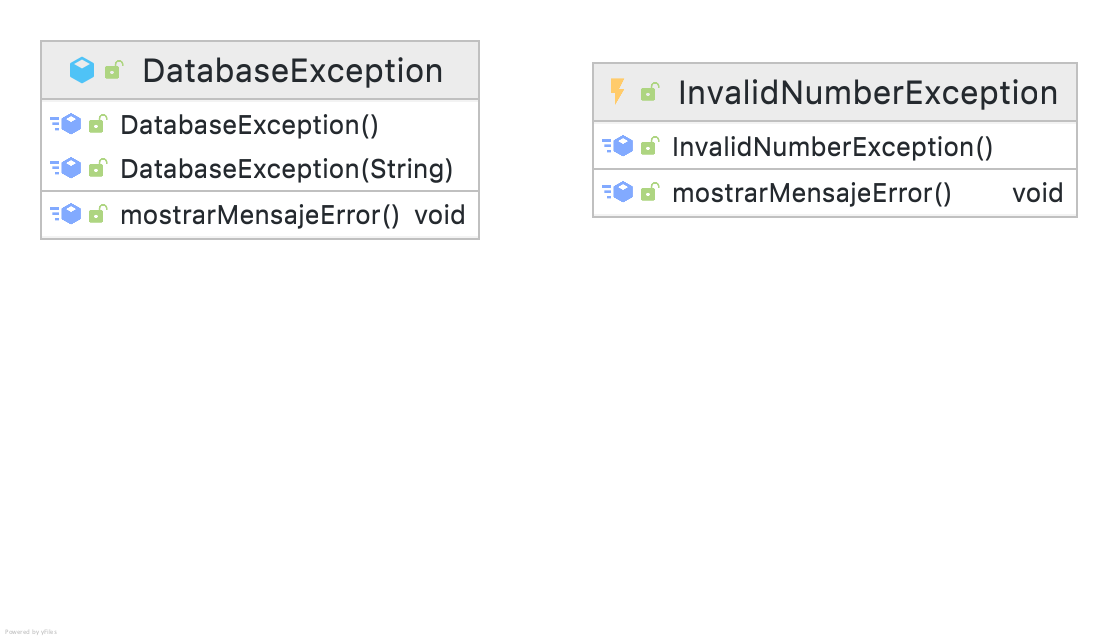
\includegraphics[width=0.75\textwidth]{contents/img/img15}
    \caption{Clases que extieden a Exception}
    \label{fig:img15}
\end{figure}

Según las funcionalidades incorporadas en el desarrollo de la solución, se hizo pertinente generar 2 clases que extienden a \textbf{Exception}:

\begin{itemize}
    \item \mintinline{java}{public class InvalidNumberException extends NumberFormatException}: Esta excepción permite capturar errores al intentar transformar una cadena de texto (ingresada por el usuario), a un típo de dato numérico (utilizando \mintinline{java}{Integer.parseInt()})
    \item \mintinline{java}{public class DatabaseException extends SQLException}: Esta excepción permite capturar errores al intentar conectarse a la base de datos MySQL
\end{itemize}

Ambas clases contienen el método \mintinline{java}{mostrarMensajeError()}, que mostrará al usuario un mensaje de error, indicandolo.

\subsection{Aplicación del patrón de diseño Strategy (Estrategia)}

En el desarrollo de la aplicación, se utilizó el patrón de diseño \textbf{Strategy} para gestionar el origen de datos del software. El uso de las interfaces presentes en el paquete \textbf{Data} contiene los métodos necesarios para obtener los datos a partir de cualquiera sea el origen de estos, lo que es aprovechado por las clases \textbf{Datafile} y \textbf{Database}, las que obtienen los datos desde archivo CSV y base de datos MySQL, respectivamente.

\clearpage

\subsubsection*{Opcional: Reemplazar los datos iniciales en el código por una conexión con base de datos local (MySQL), archivo de texto CSVo Excel, para la persistencia de datos}
\addcontentsline{toc}{subsubsection}{Opcional: Reemplazar los datos iniciales en el código por una conexión con base de datos local (MySQL), archivo de texto CSVo Excel, para la persistencia de datos}

Para la preservación de los datos poseemos tanto una carpeta en el proyecto (\textbf{Datafile}) con archivos csv, que nos permite el manejo de datos en formato local. Y también tenemos una conexión a una base de datos (\textbf{MySQL})

\begin{figure}[h]
    \centering
    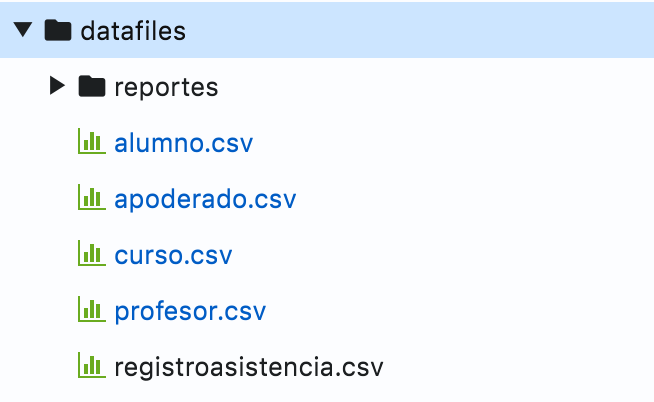
\includegraphics[width=0.35\textwidth]{contents/img/img12}
    \caption{Gestión de archivos CSV}
    \label{fig:img12}
\end{figure}

\begin{figure}[h]
    \centering
    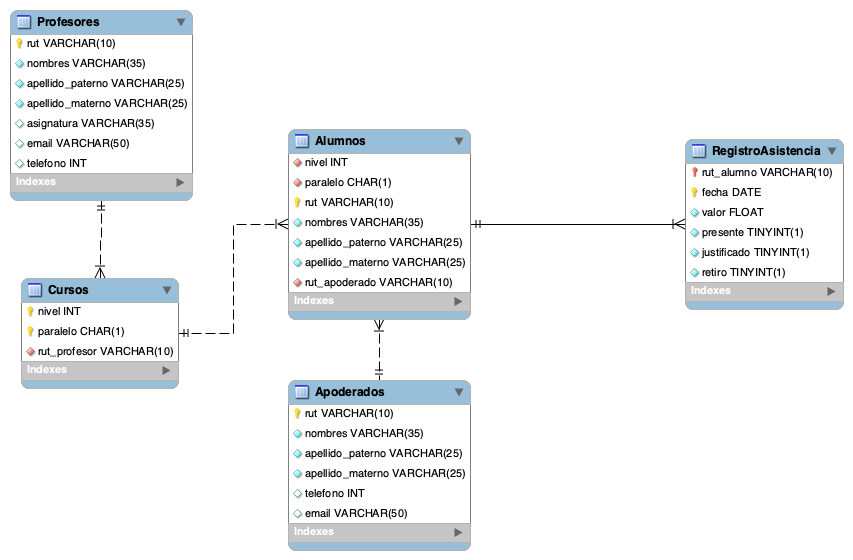
\includegraphics[width=0.85\textwidth]{contents/img/img13}
    \caption{Modelo de datos BD}
    \label{fig:img13}
\end{figure}

\clearpage

\subsubsection*{Opcional: Considerar la implementación del patrón Modelo-Vista-Controlador (MVC) en la arquitectura del sistema}
\addcontentsline{toc}{subsubsection}{Opcional: Considerar la implementación del patrón Modelo-Vista-Controlador (MVC) en la arquitectura del sistema}

Nuestro programa como se puede apreciar en la siguiente imagen  esta estructurado en un formato de modularización, en el cual separamos las clases y sus paquetes correspondientes  en un patrón MVC (Modelo-Vista-Controlador).

\begin{figure}[h]
    \centering
    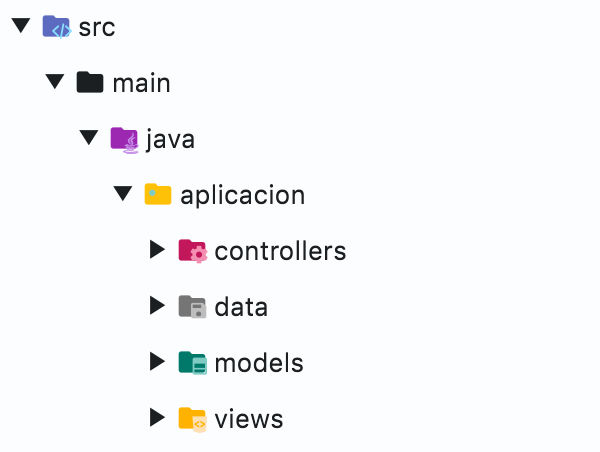
\includegraphics[width=0.35\textwidth]{contents/img/img14}
    \caption{Gestión de archivos para modelo MVC}
    \label{fig:img14}
\end{figure}
